\documentclass[12pt,a4paper]{report}
\usepackage[T2A]{fontenc}
\usepackage[utf8]{inputenc}
\usepackage[russian]{babel}
\usepackage{graphicx, setspace}

\usepackage[
top = 1.25cm, 
bottom = 2.0cm]{geometry}

\begin{document}
\begin{titlepage} 
	\centering
    % HEADER
	{
        \scshape
        Федеральное государственное автономное образовательное учреждение высшего образования
        \par
        \textbf{«Научно-образовательная корпорация ИТМО»}
        \par
        \vspace*{1cm}
        Факультет Программной Инженерии и Компьютерной Техники
        \par
    }
    % LOGO
    \vspace*{0.6cm}
    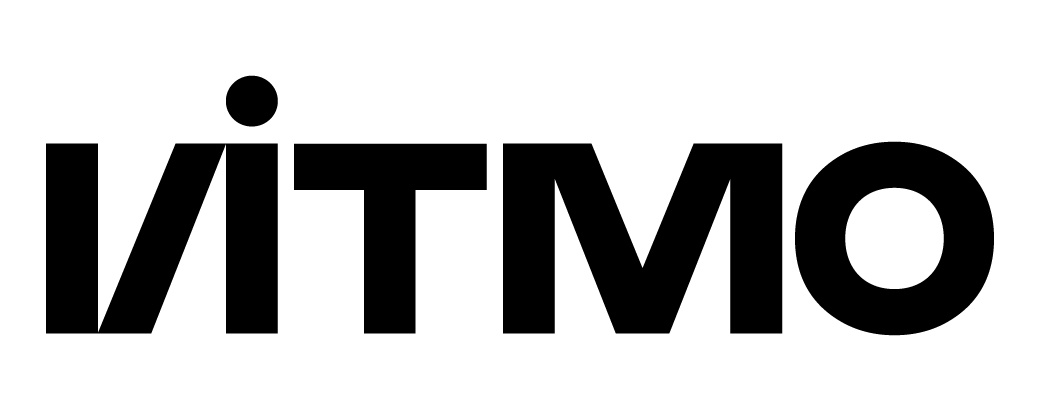
\includegraphics[width=\textwidth]{logo.png}
    % LAB INFO
    {
        \Large
        \textbf{Лабораторная работа по ОПД №7}
        \par
        \normalsize
        \vspace*{0.75cm}
        \textbf{Вариант 975}
        \par
    }
    \vfill
    % СREDITS
    \hfill\begin{minipage}{\dimexpr\textwidth-7.8cm}
        \textbf{Выполнил:}\par
        Степанов Арсений Алексеевич\par
        \vspace*{0.15cm}
        \textbf{Группа:}\par
        P3109\par
        \vspace*{0.15cm}
        \textbf{Преподаватель:}\par
        Ткешелашвили Нино Мерабиевна\par
    \end{minipage}
    \vfill
    Санкт-Петербург, \the\year{}г.
\end{titlepage}  
\section*{Задание}
Синтезировать цикл исполнения для выданных преподавателем команд. Разработать тестовые программы, которые проверяют каждую из синтезированных команд. Загрузить в микропрограммную память БЭВМ циклы исполнения синтезированных команд, загрузить в основную память БЭВМ тестовые программы. Проверить и отладить разработанные тестовые программы и микропрограммы.
\begin{itemize}
    \item ANDSP - Логическое И двух верхних чисел на вершине стека, результат поместить на стек, установить признаки N/Z
    \item Код операции - 0F10
    \item Тестовая программа должна начинаться с адреса 0389
\end{itemize}
\section*{Микрокоды новой команды}
\begin{tabular}{|c|c|c|}
    \hline
    Адр. & Код & Пояснение \\
    \hline
    BB & 81e1014002 & if CR(8) = 1 then GOTO ANDSP @ E1 \\
    \hline
    \hline
    E0 & 0080009008 & SP → AR \\
    \hline
    E1 & 0100000000 & MEM(AR) → DR \\
    \hline
    E2 & 0020009001 & DR → BR \\
    \hline
    E3 & 0080009408 & SP + 1 → AR \\
    \hline
    E4 & 0100000000 & MEM(AR) → DR \\
    \hline
    E5 & 0020809821 & BR \& DR → BR, N, Z \\
    \hline
    E6 & 0088009208 & ~0 + SP → SP, AR \\
    \hline
    E7 & 0001009020 & BR → DR \\
    \hline
    E8 & 0200000000 & DR → MEM(AR) \\
    \hline
    E9 & 80c4101040 & GOTO INT @ C4 \\
    \hline
\end{tabular}
\section*{Тестовый комплекс}
\begin{verbatim}
    ORG  0x370

    RESULT: WORD 0x0
    
    CHECK1: WORD 0x0
    CHECK2: WORD 0x0
    CHECK3: WORD 0x0
    
    RES1: WORD 0x0
    RES2: WORD 0x0FF0
    RES3: WORD 0x0320
    
    ARG1: WORD 0x0
    ARG2: WORD 0x0
    
    ARG3: WORD 0x0FFF
    ARG4: WORD 0xFFF0
    
    ARG5: WORD 0x5326
    ARG6: WORD 0x8B70
    
    ORG 0x389
    START:  CALL TEST1
            CALL TEST2
            CALL TEST3
            LD #0x1
            AND CHECK1
            AND CHECK2
            AND CHECK3
            ST RESULT
    STOP:   HLT 
    
    TEST1:  LD ARG1
            PUSH
            LD ARG2
            PUSH
            LD #0x77
            WORD 0x0F10 ; ANDSP
            CMP #0x77
            BNE ERROR1
            POP
            ST CHECK1
            CMP RES1
            BEQ DONE1
    ERROR1: POP
            POP
            CLA
            RET
    DONE1:  POP 
            POP 
            LD #0x1
            ST CHECK1
            CLA 
            RET 
    
    TEST2:  LD ARG3
            PUSH
            LD ARG4
            PUSH
            LD #0x77
            WORD 0x0F10 ; ANDSP
            CMP #0x77
            BNE ERROR2
            POP
            ST CHECK2
            CMP RES2
            BEQ DONE2
    ERROR2: POP
            POP
            CLA
            RET
    DONE2:  POP 
            POP 
            LD #0x1
            ST CHECK2
            CLA 
            RET 
    
    TEST3:  LD ARG5
            PUSH
            LD ARG6
            PUSH
            LD #0x77
            WORD 0x0F10 ; ANDSP
            CMP #0x77
            BNE ERROR3
            POP
            ST CHECK3
            CMP RES3
            BEQ DONE3
    ERROR3: POP
            POP
            CLA
            RET
    DONE3:  POP 
            POP 
            LD #0x1
            ST CHECK3
            CLA 
            RET 
    END
\end{verbatim}
\section*{Вывод}
Я понял как устроена работа базовой ЭВМ на самом низком уровне: микрокомандах, и научился использовать их в своих целях
\end{document}